\documentclass[12pt]{article}
\usepackage[utf8]{inputenc}
\usepackage{graphicx}

\usepackage[linesnumbered,ruled,vlined]{algorithm2e}

\usepackage{geometry}
\geometry{margin=2.5cm}
\usepackage{titlesec}
\titleformat{\section}{\large\bfseries}{\thesection}{1em}{}

\begin{document}

\section*{Understanding the Structure of Linearizability Testers}

This note explains three key ideas in the code from 
Gavin Lowe: the concept of a \textit{companion object},
 the idea of a \textit{factory of testers}, and a
  high-level overview of the UML diagram about its code.

\section{Companion Object}
In Scala, a \textbf{companion object} is 
an \texttt{object} that has the same name as a \texttt{class}. 
It lives in the same source file and 
can access the class’s private members. 

The difference is simple:
\begin{itemize}
  \item The \texttt{class} defines how to create \textbf{instances}.
  \item The \texttt{object} defines 
  \textbf{static methods or values}, similar to \texttt{static} in Java.
\end{itemize}

So, when we see \texttt{object LinearizabilityTester}, 
it is the companion of the class \texttt{LinearizabilityTester}. 
It is not an instance, but a place to store reusable methods that help build testers.

\section{Factory of Testers}
The companion object is used as a \textbf{factory}.
 This means it provides methods to create ready-made
  testers without the user needing to wire everything together. 

Instead of writing all details manually,
 such as which log to use and which solver
  to instantiate, we can call:
\begin{verbatim}
LinearizabilityTester.JITTree(seqObj, concObj, p, worker, iters)
\end{verbatim}

This automatically produces a \texttt{LinearizabilityTester} configured with:
\begin{itemize}
  \item the right kind of log (\texttt{SharedLog} or \texttt{TSLog}),
  \item and the right solver (\texttt{JITLinUndoTester}, \texttt{WGGraph}, etc.).
\end{itemize}

This is called a \textit{factory pattern}, 
and it hides complex setup code behind a clean and simple interface.

\newpage

\section{High-Level UML Description}



\begin{figure}[htbp]
        \begin{center}
            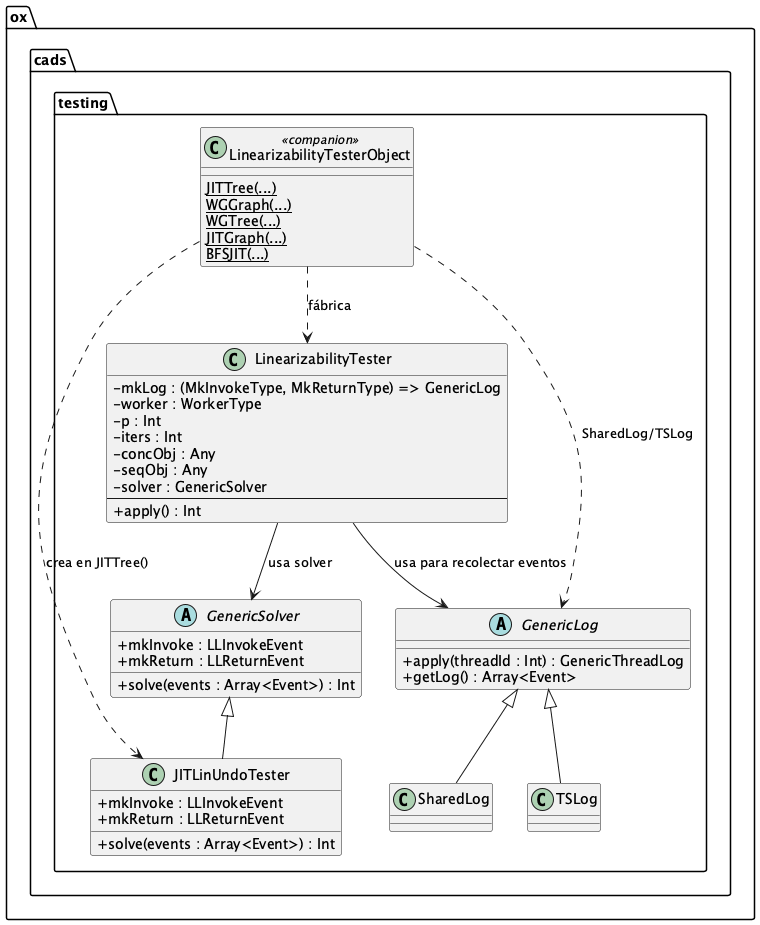
\includegraphics[width=0.74\textwidth]{../uml/LinTester2.png}
        \caption{UML diagram at a high level}\label{fig:uml-highlevel}
        \end{center}
\end{figure}

The UML diagram in Figure~\ref{fig:uml-highlevel} shows 
the main building blocks and how they are connected:

\begin{itemize}
  \item \textbf{LinearizabilityTester} is the
   central harness. 
   It brings together a concurrent object,
    a sequential specification, a log, and a solver.
  \item The \textbf{logs} (\texttt{SharedLog}, \texttt{TSLog}) 
  are responsible for recording what operations threads do. 
  They provide thread-specific logs (\texttt{SharedThreadLog}, \texttt{TSThreadLog}).
  \item The \textbf{solver} (like \texttt{JITLinUndoTester})
   is the algorithm that checks if the recorded execution is linearizable.
  \item The \textbf{companion object} 
  \texttt{LinearizabilityTester} acts as a factory.
   It has methods (\texttt{WGGraph}, \texttt{WGTree}, 
   \texttt{JITTree}, etc.) that build different
    kinds of testers by combining a log and a solver.
  \item Supporting classes like \texttt{UndoConfig} 
  and \texttt{Event}/\texttt{ReturnEvent} 
  are used internally by solvers to represen
  t states and histories.
\end{itemize}



At a high level, the picture is:
\begin{quote}
The \texttt{LinearizabilityTester} uses a \textbf{log} to collect events, then passes those events to a \textbf{solver} that decides if the execution is linearizable.
The companion object makes it easy to create testers with different solvers and logs.
\end{quote}

\section{JITLinUndoTester}

	The Just-In-Time Linearizability Tester (JITLinUndoTester)
   is a tool designed to check if the behavior of a concurrent object
    is linearizable with respect to a given sequential specification.
    The key idea is to explore all possible linearization 
    orders of concurrent operations using backtracking, 
    while undoing invalid attempts, 
    to decide whether a given execution history is linearizable.

	It relies on:
  \begin{enumerate}
    \item Just-in-time linearization: Operations are only linearized 
    when necessary, allowing flexibility in exploring possible orders.
	  \item Depth-first tree search: The algorithm recursively 
    (or iteratively) explores all possible linearization orders of concurrent events.
	  \item Undoable sequential specification object:
     The sequential object can be “undone” (rolled back) 
     after tentative linearizations, enabling efficient backtracking when a path fails.
  \end{enumerate}

	The tester supports two solving strategies:
	A recursive version, which is easier to understand but limited by stack depth.
	An iterative version, which explicitly manages its own stack
   and avoids stack overflow on long histories.
	
  For each event in the execution history:
  \begin{itemize}
    \item Invoke events are recorded as pending operations.
	  \item Return events are only accepted if the operation has
   already been linearized; otherwise, the tester
    attempts to fire pending operations in different
     orders until consistency is achieved.
  \end{itemize}
	The tester provides debugging output:
	Tracks how far it managed to linearize the history (to ``remember'').
	Reports the allowed results for return events when a mismatch occurs.
	
\begin{algorithm}[H]
\caption{Pseudocode of the Recursive Solver version in JITLinUndoTester with UndoConfig}
\SetKwFunction{Fsolve}{solve}
\SetKwFunction{FfireOthersThen}{fireOthersThen}

\SetKwProg{Fn}{Function}{:}{}
\Fn{\Fsolve{$i$}}{
    \tcp{Base case: all events processed}
    \If{$i =$ length$($events$)$}{
        \Return SUCCESS
    }

    $event \gets events[i]$\;

    \uIf{$event$ is InvokeEvent$(t, msg, op)$}{
        \tcp{1. Record invocation in UndoConfig (Out $\to$ Pending)}
        config.invoke($t, msg, op, event.expectedResult$)\;

        \tcp{2. Recurse to process next event}
        $result \gets$ \Fsolve{$i+1$}\;

        \If{$result \neq$ FAILURE}{
            \Return $result$
        }
        \Else{
            \tcp{3. Backtrack if failed (Pending $\to$ Out)}
            config.uninvoke($t, msg, op, event.expectedResult$)\;
            \Return FAILURE
        }
    }
    \uElseIf{$event$ is ReturnEvent$(t, result)$}{
        \If{config.canReturn($t$)}{
            \tcp{1. Operation already linearized (Ret $\to$ Out)}
            $prev \gets$ config.doReturn($t$)\;

            \tcp{2. Recurse on next event}
            $result \gets$ \Fsolve{$i+1$}\;

            \If{$result \neq$ FAILURE}{
                \Return $result$
            }
            \Else{
                \tcp{3. Backtrack: restore previous Ret state}
                config.undo($t, prev$)\;
                \Return FAILURE
            }
        }
        \Else{
            \tcp{Cannot return yet: must try to linearize other pending ops}
            \Return \FfireOthersThen{$t, i$}
        }
    }
}

\end{algorithm}

\newpage  % --- Force new page ---

\begin{algorithm}[H]
\caption{Helper Function: \texttt{fireOthersThen(t, i)}}
\SetKwFunction{Fsolve}{solve}
\SetKwFunction{FfireOthersThen}{fireOthersThen}


\SetKwProg{Fn}{Function}{:}{}
\Fn{\FfireOthersThen{$t, i$}}{
    \tcp{Iterate over all threads: start with $t$, then 0..p-1 (except $t$)}
    \ForEach{thread $t1$}{
        \If{config.hasPending($t1$) or $t1 = t$}{
            \tcp{Try to fire the pending operation}
            $outcome \gets$ \uIf{$t1 = t$}{config.fireRet($t1$)} \Else{config.fire($t1$)}\;

            \uIf{$outcome$ is Left(prevState)}{
                \tcp{Fire succeeded: continue searching }
                $result \gets$ \uIf{$t1 = t$}{\Fsolve{$i+1$}} \Else{\FfireOthersThen{$t, i$}}\;

                \If{$result \neq$ FAILURE}{
                    \Return $result$
                }
                \Else{
                    \tcp{Backtrack: undo firing}
                    config.undo($t1, prevState$)\;
                }
            }
            \Else{
                \tcp{Fire failed: record allowed results, try next thread}
                recordAllowedResult($t1, outcome$)\;
            }
        }
    }
    \tcp{If no ordering works, return failure}
    \Return FAILURE
}

\end{algorithm}

\end{document}
